\documentclass{lab_sheet}
\usepackage{longtable}
\usepackage{mathtools}
\usepackage{hyperref}
\def\ddfrac#1#2{\displaystyle\frac{\displaystyle #1}{\displaystyle #2}}
\usetikzlibrary{shapes.geometric, arrows, decorations.markings}
\tikzstyle{rect} = [rectangle, rounded corners, minimum width=2cm, minimum height=1cm,text centered, draw=black, fill=blue!10]
\tikzstyle{blank} = [rectangle]
\tikzstyle{arrow} = [->,>=stealth]
\tikzstyle{mCircle}=[circle, draw=black, fill=blue!10]


\newcommand{\ltisystem}{
    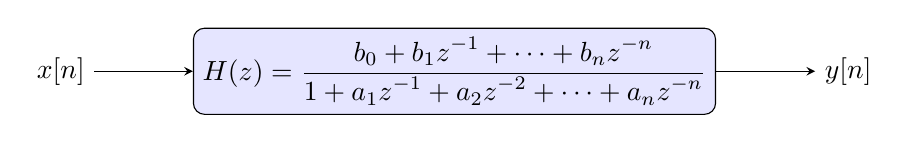
\begin{tikzpicture}[node distance=5 cm]
    \node (lti) [rect] {$H(z)=\ddfrac{b_0+b_1z^{-1}+\dots+b_nz^{-n}}{1+a_1z^{-1}+a_2z^{-2}+\dots+a_nz^{-n}}$};
    \node (b1) [blank, left of=lti] {$x[n]$};
    \node (b2) [blank, right of=lti] {$y[n]$};
    \draw [arrow] (b1.east) -- (lti.west);
    \draw [arrow] (lti.east) -- (b2);
    \end{tikzpicture}
    }

    \newcommand{\cascade}{
    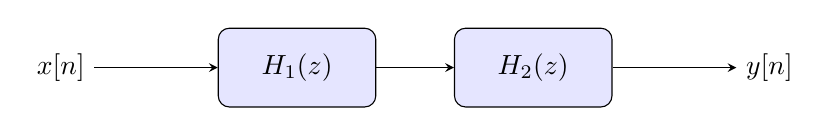
\begin{tikzpicture}[node distance=3 cm]
    \node (c1) [rect] at (0,0) {$H_1(z)$};
    \node (c2) [rect, right of=c1] {$H_2(z)$};
    \node (b1) [blank, left of=c1] {$x[n]$};
    \node (b2) [blank, right of=c2] {$y[n]$};
    \draw [arrow] (b1.east) -- (c1.west);
    \draw [arrow] (c1.east) -- (c2.west);
    \draw [arrow] (c2.east) -- (b2.west);
    \end{tikzpicture}
    }

    \newcommand{\sfg}{
    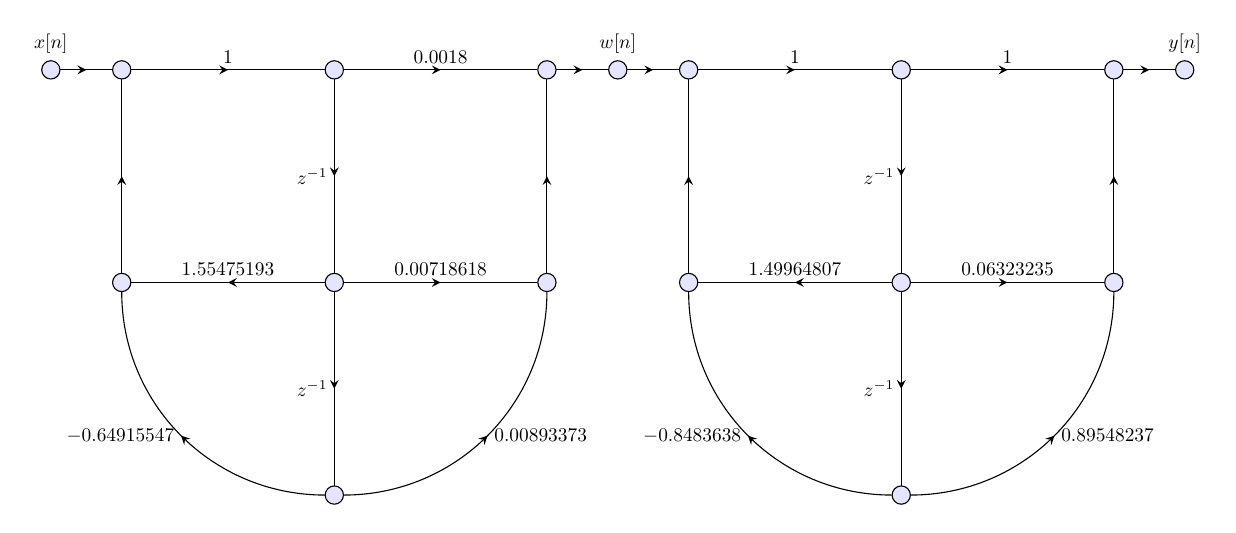
\begin{tikzpicture}[midarrow/.style={decoration={markings, mark=at position 0.5 with {\arrow{stealth}}},postaction={decorate}}, every node/.style={scale=0.7},scale=0.9]
        \node[mCircle, label={$x[n]$}] (m1) at (-4,0) {};
        \node[mCircle] (m2) at (-3,0) {};
        \node[mCircle] (m3) at (0,0) {};
        \node[mCircle] (m4) at (3,0) {};
        \node[mCircle,label={$w[n]$}] (m5) at (4,0) {};
        \node[mCircle] (m6) at (-3,-3) {};
        \node[mCircle] (m7) at (0,-3) {};
        \node[mCircle] (m8) at (3,-3) {};
        \node[mCircle] (m9) at (0,-6) {};

        \node[mCircle] (n2) at (5,0) {};
        \node[mCircle] (n3) at (8,0) {};
        \node[mCircle] (n4) at (11,0) {};
        \node[mCircle,label={$y[n]$}] (n5) at (12,0) {};
        \node[mCircle] (n6) at (5,-3) {};
        \node[mCircle] (n7) at (8,-3) {};
        \node[mCircle] (n8) at (11,-3) {};
        \node[mCircle] (n9) at (8,-6) {};

        \draw[midarrow] (m1) -- (m2);
        \draw[midarrow] (m2) -- node[above] {$1$} (m3);
        \draw[midarrow] (m3) -- node[above] {$0.0018$} (m4);
        \draw[midarrow] (m4) -- (m5);

        \draw[midarrow] (m3) -- node[left] {$z^{-1}$} (m7);
        \draw[midarrow] (m7) -- node[left] {$z^{-1}$} (m9);

        \draw[midarrow] (m7) -- node[above] {$1.55475193$} (m6);
        \draw[midarrow] (m7) -- node[above] {$0.00718618$} (m8);
        \draw[midarrow] (m8) -- (m4);
        \draw[midarrow] (m6) -- (m2);

        \draw[midarrow,looseness=1] (m9) to[out=180,in=270] node[left] {$-0.64915547$} (m6);
        \draw[midarrow,looseness=1] (m9) to[out=0,in=270] node[right] {$0.00893373$} (m8);
        
        \draw[midarrow] (m5) -- (n2);
        \draw[midarrow] (n2) -- node[above] {$1$} (n3);
        \draw[midarrow] (n3) -- node[above] {$1$} (n4);
        \draw[midarrow] (n4) -- (n5);

        \draw[midarrow] (n3) -- node[left] {$z^{-1}$} (n7);
        \draw[midarrow] (n7) -- node[left] {$z^{-1}$} (n9);

        \draw[midarrow] (n7) -- node[above] {$1.49964807$} (n6);
        \draw[midarrow] (n7) -- node[above] {$0.06323235$} (n8);
        \draw[midarrow] (n8) -- (n4);
        \draw[midarrow] (n6) -- (n2);

        \draw[midarrow,looseness=1] (n9) to[out=180,in=270] node[left] {$-0.8483638$} (n6);
        \draw[midarrow,looseness=1] (n9) to[out=0,in=270] node[right] {$0.89548237$} (n8);
        \end{tikzpicture}
    }

\newcommand{\directi}{
    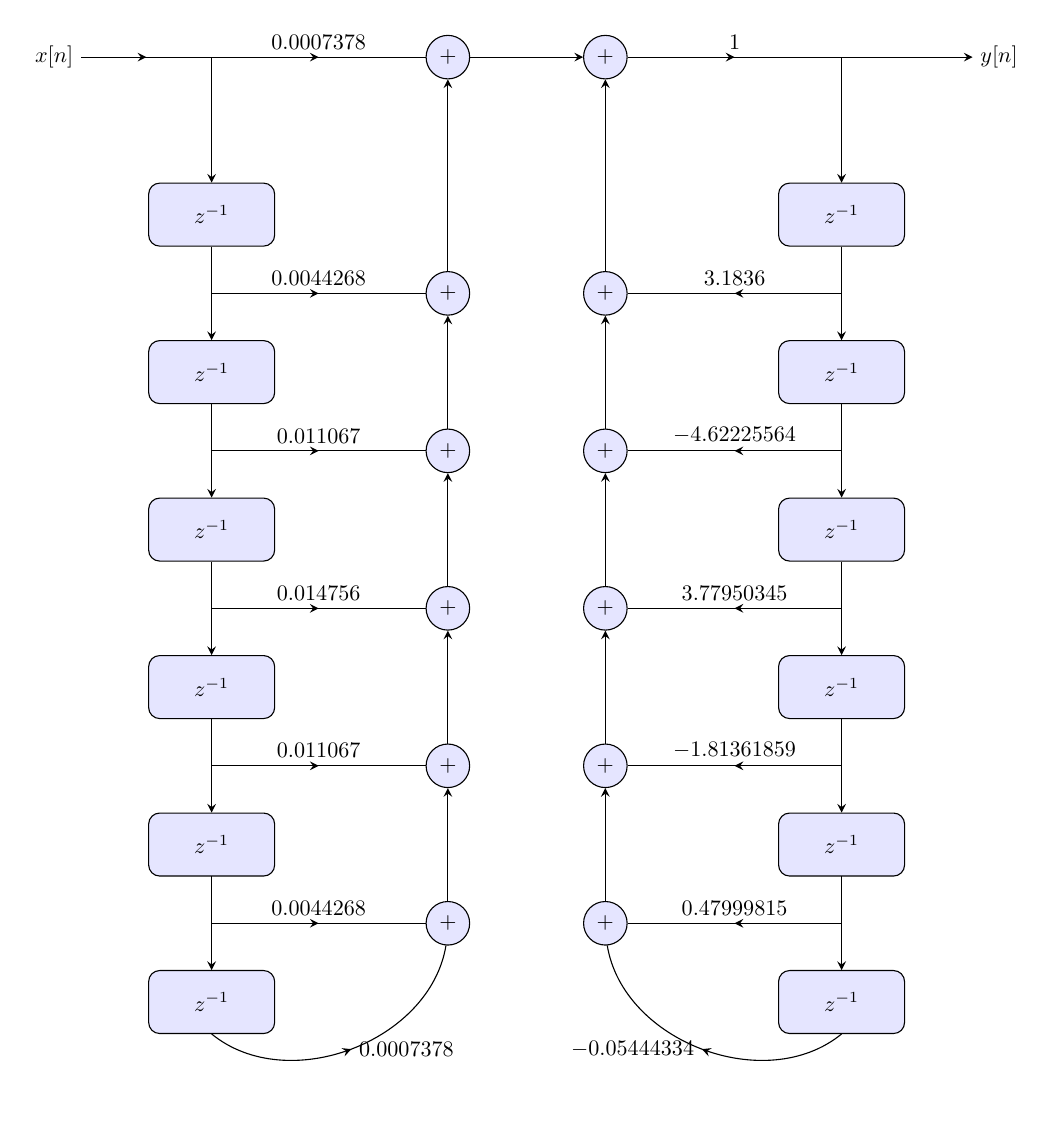
\begin{tikzpicture}[midarrow/.style={decoration={markings, mark=at position 0.5 with {\arrow{stealth}}},postaction={decorate}}, every node/.style={scale=0.8},scale=1]
        \node[blank] (x) at (-6,0) {$x[n]$};
        \foreach \j in {-2,-4,...,-12}
        {\node[rect] (x\j) at (-4,\j) {$z^{-1}$};}

        \node[mCircle] (xs) at (-1,0) {$+$};
        \foreach \j in {-3,-5,...,-11}
        {\node[mCircle] (xs\j) at (-1,\j) {$+$};}

        \node[mCircle] (ys) at (1,0) {$+$};
        \foreach \j in {-3,-5,...,-11}
        {\node[mCircle] (ys\j) at (1,\j) {$+$};}

        \node[blank] (y) at (6,0) {$y[n]$};
        \foreach \j in {-2,-4,...,-12}
        {\node[rect] (y\j) at (4,\j) {$z^{-1}$};}

        \draw [midarrow] (x)--(-4,0);
        \draw [midarrow] (-4,0)--node[above] {$0.0007378$}(xs);
        \draw[arrow] (xs)--(ys);
        \draw[midarrow] (ys)--node[above] {$1$} (4,0) ;
        \draw[arrow] (4,0)--(y) ;

        \draw[arrow] (-4,0)--(x-2.north);
        \draw[arrow] (x-2.south)--(x-4.north);
        \draw[arrow] (x-4.south)--(x-6.north);
        \draw[arrow] (x-6.south)--(x-8.north);
        \draw[arrow] (x-8.south)--(x-10.north);
        \draw[arrow] (x-10.south)--(x-12.north);
        \draw[midarrow] (-4,-3) -- node[above] {$0.0044268$} (xs-3);
        \draw[midarrow] (-4,-5) -- node[above] {$0.011067$} (xs-5);
        \draw[midarrow] (-4,-7) -- node[above] {$0.014756$} (xs-7);
        \draw[midarrow] (-4,-9) -- node[above] {$0.011067$} (xs-9);
        \draw[midarrow] (-4,-11) -- node[above] {$0.0044268$} (xs-11);
        \draw[midarrow] (x-12.south) to[bend right=60] node[right] {$0.0007378$} (xs-11);
        \draw [arrow] (xs-11)--(xs-9);
        \draw [arrow] (xs-9)--(xs-7);
        \draw [arrow] (xs-7)--(xs-5);
        \draw [arrow] (xs-5)--(xs-3);
        \draw [arrow] (xs-3)--(xs);

        \draw[arrow] (4,0)--(y-2.north);
        \draw[arrow] (y-2.south)--(y-4.north);
        \draw[arrow] (y-4.south)--(y-6.north);
        \draw[arrow] (y-6.south)--(y-8.north);
        \draw[arrow] (y-8.south)--(y-10.north);
        \draw[arrow] (y-10.south)--(y-12.north);
        \draw[midarrow] (4,-3) -- node[above] {$3.1836$} (ys-3);
        \draw[midarrow] (4,-5) -- node[above] {$-4.62225564$} (ys-5);
        \draw[midarrow] (4,-7) -- node[above] {$3.77950345$} (ys-7);
        \draw[midarrow] (4,-9) -- node[above] {$-1.81361859$} (ys-9);
        \draw[midarrow] (4,-11) -- node[above] {$0.47999815$} (ys-11);
        \draw[midarrow] (y-12.south) to[bend left=60] node[left] {$-0.05444334$} (ys-11);
        \draw [arrow] (ys-11)--(ys-9);
        \draw [arrow] (ys-9)--(ys-7);
        \draw [arrow] (ys-7)--(ys-5);
        \draw [arrow] (ys-5)--(ys-3);
        \draw [arrow] (ys-3)--(ys);
        \end{tikzpicture}
    }

    \newcommand{\directii}{
    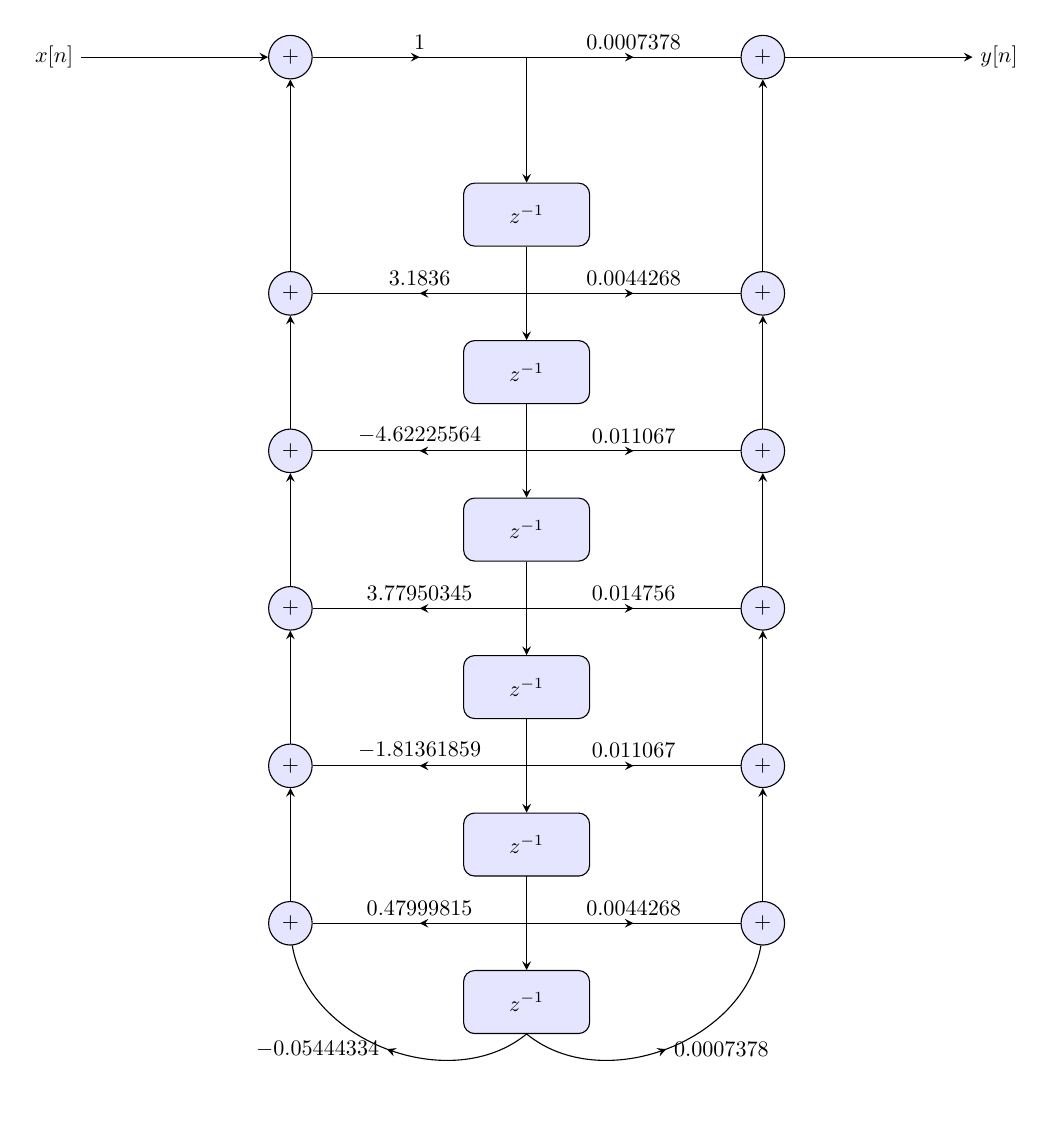
\begin{tikzpicture}[midarrow/.style={decoration={markings, mark=at position 0.5 with {\arrow{stealth}}},postaction={decorate}}, every node/.style={scale=0.8},scale=1]
        \node[blank] (x) at (-6,0) {$x[n]$};
        \foreach \j in {-2,-4,...,-12}
        {\node[rect] (x\j) at (0,\j) {$z^{-1}$};}

        \node[mCircle] (xs) at (3,0) {$+$};
        \foreach \j in {-3,-5,...,-11}
        {\node[mCircle] (xs\j) at (3,\j) {$+$};}

        \node[mCircle] (ys) at (-3,0) {$+$};
        \foreach \j in {-3,-5,...,-11}
        {\node[mCircle] (ys\j) at (-3,\j) {$+$};}

        \node[blank] (y) at (6,0) {$y[n]$};

        \draw[arrow](x)--(ys);
        \draw [midarrow] (ys)--node[above] {$1$}(0,0);
        \draw[midarrow] (0,0)--node[above] {$0.0007378$}(xs);
        \draw[arrow](xs)--(y);
        \draw[arrow] (0,0)--(x-2.north);
        \draw[arrow] (x-2.south)--(x-4.north);
        \draw[arrow] (x-4.south)--(x-6.north);
        \draw[arrow] (x-6.south)--(x-8.north);
        \draw[arrow] (x-8.south)--(x-10.north);
        \draw[arrow] (x-10.south)--(x-12.north);
        \draw[midarrow] (0,-3) -- node[above] {$0.0044268$} (xs-3);
        \draw[midarrow] (0,-5) -- node[above] {$0.011067$} (xs-5);
        \draw[midarrow] (0,-7) -- node[above] {$0.014756$} (xs-7);
        \draw[midarrow] (0,-9) -- node[above] {$0.011067$} (xs-9);
        \draw[midarrow] (0,-11) -- node[above] {$0.0044268$} (xs-11);
        \draw[midarrow] (x-12.south) to[bend right=60] node[right] {$0.0007378$} (xs-11);
        \draw [arrow] (xs-11)--(xs-9);
        \draw [arrow] (xs-9)--(xs-7);
        \draw [arrow] (xs-7)--(xs-5);
        \draw [arrow] (xs-5)--(xs-3);
        \draw [arrow] (xs-3)--(xs);

        \draw[midarrow] (0,-3) -- node[above] {$3.1836$} (ys-3);
        \draw[midarrow] (0,-5) -- node[above] {$-4.62225564$} (ys-5);
        \draw[midarrow] (0,-7) -- node[above] {$3.77950345$} (ys-7);
        \draw[midarrow] (0,-9) -- node[above] {$-1.81361859$} (ys-9);
        \draw[midarrow] (0,-11) -- node[above] {$0.47999815$} (ys-11);
        \draw[midarrow] (x-12.south) to[bend left=60] node[left] {$-0.05444334$} (ys-11);
        \draw [arrow] (ys-11)--(ys-9);
        \draw [arrow] (ys-9)--(ys-7);
        \draw [arrow] (ys-7)--(ys-5);
        \draw [arrow] (ys-5)--(ys-3);
        \draw [arrow] (ys-3)--(ys);
        \end{tikzpicture}
    }
\begin{document}
\titlePage{Linear Time Invariant System}{January 16, 2022}
\pagenumbering{roman}
\clearpage
\tableofcontents
\clearpage
\phantomsection
\addcontentsline{toc}{section}{\bfseries{List of Figures}}
\listoffigures
\clearpage
\phantomsection
\addcontentsline{toc}{section}{\bfseries{Listings}}
\lstlistoflistings
\clearpage
\pagenumbering{arabic}
\section{Objectives}
\begin{itemize}
	\item Familiarization with linear system transformations and response visualization.
	\item Familiarization with second order section representation of LTI system.
\end{itemize}
\section{Background Theory}
\subsection{Linear Time Invariant (LTI) System}
\begin{figure}[H]
	\centering
	\ltisystem
	\caption{LTI system with transfer function $H(z)$}
	\label{fig:lti_system}
\end{figure}
A linear time invariant (LTI)system is characterized by the transfer function $H(z)=\ddfrac{Y(z)}{X(z)}$,
where $X(z)$ and $Y(z)$ are the Z-transforms of the sequences $x[n]$ and $y[n]$ respectively. When the
inverse Z-transform of the transfer function $H(z)$ is taken, the resulting difference equation can be written as:
\begin{equation*}
	y[n]=b_0x[n]+b_1x[n-1]+\dots+b_Nx[n-N]-a_1y[n-1]-a_2y[n-2]-\dots-a_Ny[n-N]
\end{equation*}
The digital signal processing basically deals with the methods of implementation of the above
difference equation. The equation can be solved using both hardware and software. It can be
implemented using microprocessor based designs in which the assembly language programming
plays the vital role. For the fast processing of the signals, considering the improved system
performance the digital signal processing chips are preferred. The DSP chips are based on the
Harvard architecture rather than the Von-Neumann's architecture, usually found in most of the
personal computers.\\
If the transfer function $H(z)$ is known for the given LTI system the MATLAB signal processing
toolbox functions can be used to plot the frequency response of the system. For this there is a
function;
\begin{verbatim}
    [H, W]= freqz(b, a, w)
\end{verbatim}
which gives the complex values in amplitude \texttt{H} and angle \texttt{W} radians versus w points frequency. Here \texttt{a}  and \texttt{b} are the vector sequences representing the
numerator and denominator coefficients of $H(z)$.
\subsection{Linear Systems Transformation}
In discrete time systems the transfer function in the Z domain plays the key role in determining the nature of the system. The nature of the system is determined from the number and locations of the poles and zeros in the Z-plane. In lower order systems the locations of the poles and zeros can be easily determined from the transfer function of the system. However the higher order systems possess transfer functions with numerator and denominator polynomials of greater degree. As a result the process of determining the poles and zeros of the system becomes complex and tedious. Besides this in most of the higher order discrete time systems, the transfer function is specified in the form of second order sections. If the transfer function of the system consists of a large number of such second order sections either in cascade or parallel form, the determination of the poles and zeros of the system becomes even harder.\\MATLAB signal processing toolbox provides a number of functions for transforming the discrete time linear systems from one form to another. The name of the functions and their purpose are listed as follows:
\begin{longtable}[H]
    {|m{0.2\linewidth}|m{0.7\linewidth}|}
        \hline
        \textbf{Function}&\textbf{Purpose}\\
        \hline\hline
        \texttt{sos2zp}&Transforms second order sections into zeros and poles.\\
        \hline
        \texttt{sos2tf}&Performs second order sections to transfer function conversion.\\
        \hline
        \texttt{tf2zp}&Transfer function to pole zero conversion.\\
        \hline
        \texttt{zp2sos}&Zero-poles to second order sections.\\
        \hline
        \texttt{zplane}&Plots the pole-zero diagram in Z-plane.\\
        \hline
        \texttt{freqz}&Determines the magnitude and phase of the transfer function.\\
        \hline
\end{longtable}
\textit{Note: Similar functions are available in the \texttt{Scipy} library in Python.}
\section{Lab Exercises}
\mysub{LTI system with given coefficients}
\problem{In the given LTI system of fig above, if the coefficients $b$ and $a$ are specified as,\\ $b_0=0.0663,\quad b_1=0.1989,\quad b_2=0.1989,\quad b_3=0.0663$ \\$a_0=1,\quad a_1= -0.9349,\quad a_2=0.5668,\quad a_3= -0.1015$\\then the order of the system is 3 i.e. $N=3$.}
\subproblem{Plot the frequency response of the system.}
\subproblem{From the magnitude response of the system, find out the cut-off frequency.}
\subproblem{Identify the nature of the system analyzing its frequency response.}
\pythoncode{lab_4_1}{Python script for frequency response and linearized form visualization for given coefficients}
\begin{figure}[H]
	\centering
	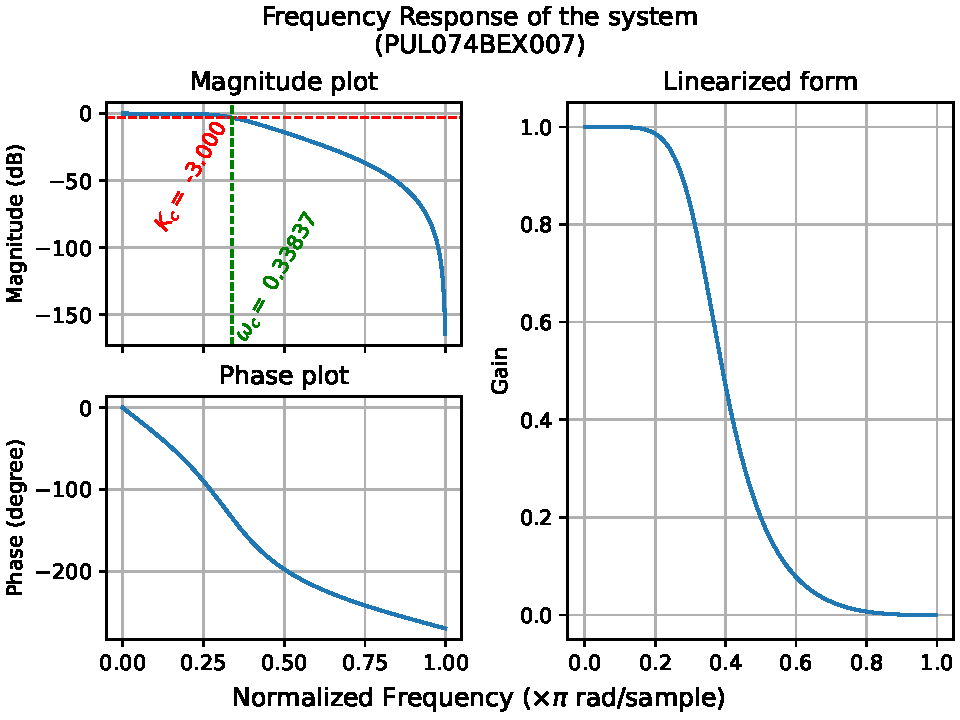
\includegraphics[width=\linewidth]{../Figures/lab_4_1_py.pdf}
	\caption{Observation of frequency response and linearized form for given coefficients}
	\label{fig:4_1_py}
\end{figure}
The frequency response for given set of coefficients is shown in Figure~\ref{fig:4_1_py}. The magnitude response has annotations added at cut-off frequency and cut-off magnitude for better result and visualization. The noted value of cut-off frequency is $\omega_c=0.33837$, which is actually in normalized form, i.e. ($\times \pi$ rad/sample). Similarly, the linearized form plot suggests that the nature of the system is low pass.
\mysub{LTI system with given transfer function}
\problem{The transfer function of the fourth-order discrete time system is given as,
\begin{equation*}
    H(z)=\frac{0.0018+0.0073z^{-1}+0.011z^{-2}+0.007z^{-3}+0.008z^{-4}}{1-3.0544z^{-1}+3.8291z^{-2}-2.2925z^{-3}+0.55072z^{-4}}
\end{equation*}}
\subproblem{Find out the poles and zeros of the system and plot them in the z- plane.}
\subproblem{Use them to determine the second order sections in the cascaded form.}
\subproblem{Plot the frequency response of the system and comment on the nature of the system.}
\subproblem{After knowing the numerator and denominator coefficients of each second order section, draw the signal flow graph to represent the cascaded structure.}
\pythoncode{lab_4_2}{Python script for determination of SOS, zero-pole plot, and linearized form visualization for given transfer function}
\begin{figure}[H]
	\centering
	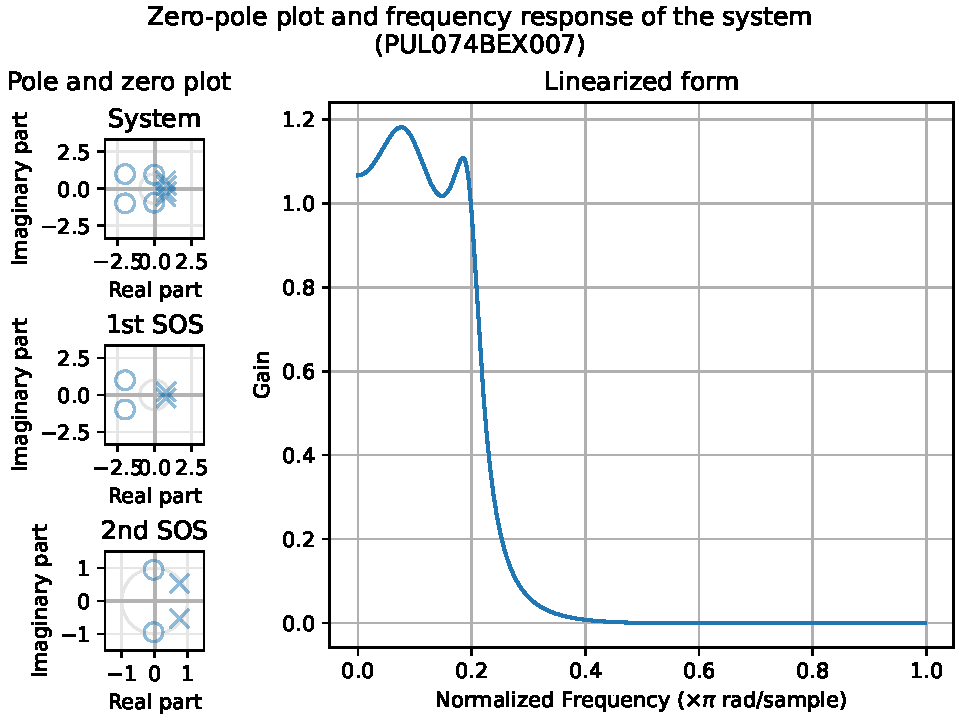
\includegraphics[width=\linewidth]{../Figures/lab_4_2_py.pdf}
	\caption{Observation of zero-pole plot and linearized form for given transfer function}
	\label{fig:4_2_py}
\end{figure}
The zero-pole plot in the Z-plane for the system, the first and second sections of the SOS are observed in Figure~\ref{fig:4_2_py}. Similarly, the linearized form plot suggests that the nature of the system is low pass. The second order sections for the given transfer function are displayed in the terminal as,
\begin{verbatim}
[[ 0.0018  0.00718618  0.00893373  1.  -1.55475193  0.64915547]
[ 1.  0.06323235  0.89548237  1.  -1.49964807  0.8483638]]
\end{verbatim}
\mysubsub{Cascade representation from determined SOS}
Upon review of the return value from \texttt{tf2sos}, each row contains one section of the SOS. Likewise, the first three values in each row represent the numerator coefficients and the remaining three values represent the denominator coefficients of that section. Hence, the two second order sections in cascade structure can be represented as,
\begin{equation*}
    H_1(z)=\frac{0.0018+0.00718618z^{-1}+0.00893373z^{-2}}{1-1.55475193z^{-1}+0.64915547z^{-2}}
\end{equation*}
\begin{equation*}
    H_2(z)=\frac{1+0.06323235z^{-1}+0.89548237z^{-2}}{1-1.49964807z^{-1}+0.8483638z^{-2}}
\end{equation*}
\begin{figure}[H]
	\centering
	\cascade
	\caption{LTI system represented as cascade of two SOS}
	\label{fig:cascade_sos_system}
\end{figure}
\begin{figure}[H]
	\centering
	\sfg
	\caption{Signal flow graph to represent the cascade structure in Figure~\ref{fig:cascade_sos_system}}
	\label{fig:sfg}
\end{figure}
\mysub{LTI system with given SOS cascade}
\problem{Let a discrete time system be implemented by cascading of the following three second order sections:\\
Section 1:
    $H_1(z)=\ddfrac{0.0007378(1+2z^{-1}+z^{-2})}{1-1.2686z^{-1}+0.7051z^{-2}}$\\
Section 2:
    $H_2(z)=\ddfrac{1+2z^{-1}+z^{-2}}{1-1.0106z^{-1}+0.3583z^{-2}}$\\
    Section 3:
    $H_3(z)=\ddfrac{1+2z^{-1}+z^{-2}}{1-0.9044z^{-1}+0.2155z^{-2}}$
}
\subproblem{Using above three second order sections in cascaded form determine the poles and
zeros of the system and plot them in z-plane.}
\subproblem{Determine the transfer function of the system, formed by cascading of the above three sections. Determine the poles and zeros from this transfer function and plot them in z-plane. Your result should match with that from previous one.}
\subproblem{Draw the direct form structures-I and II of the system.}
\pythoncode{lab_4_3}{Python script for zero-pole plot visualization for given SOS cascade}
\begin{figure}[H]
	\centering
	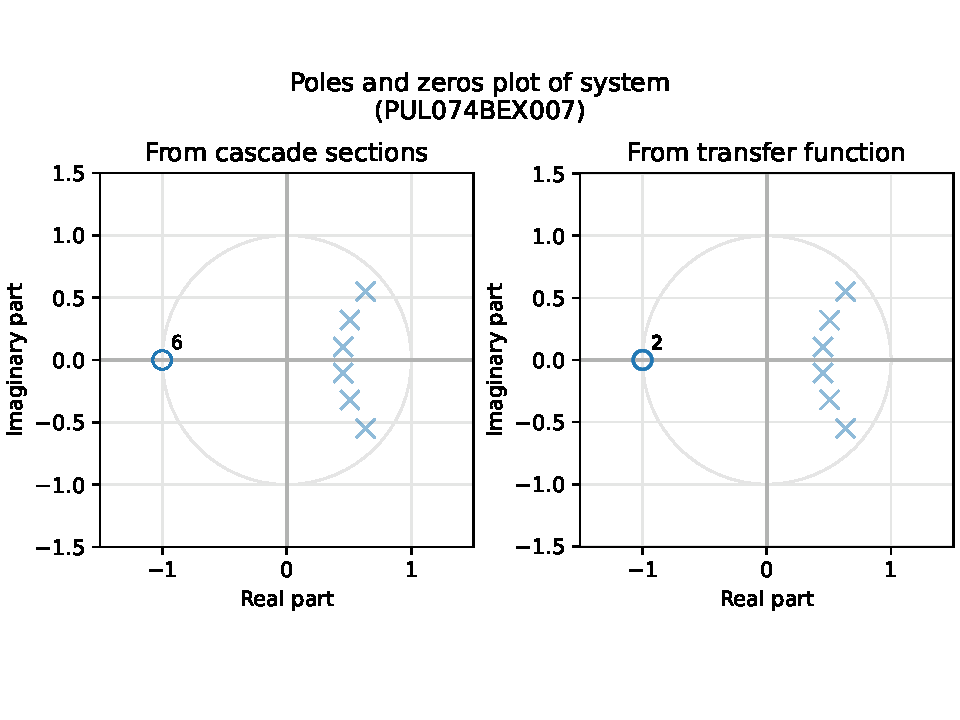
\includegraphics[width=\linewidth]{../Figures/lab_4_3_py.pdf}
	\caption{Observation of zero-pole plot for given SOS cascade}
	\label{fig:4_3_py}
\end{figure}
The zero-pole plot for cascade of three sections of SOS and the zero-pole plot from the determined transfer function is same as seen in Figure~\ref{fig:4_3_py}. Slight deviation is seen as there are $6$ zeros as same co-ordinate for the plot from cascade of sections where as there are $3$ set of $2$ poles each in same co-ordinate for the plot from transfer function, which is due to computational accuracy. The coefficients of numerator and denominator of the transfer function, $b$ and $a$ for the given cascade of three SOS are displayed in the terminal as,
\mysubsub{Direct form representations from determined transfer function}
\begin{verbatim}
    [0.0007378  0.0044268  0.011067  0.014756  0.011067  0.0044268
    0.0007378]
    [ 1.  -3.1836  4.62225564  -3.77950345  1.81361859  -0.47999815
    0.05444334]
\end{verbatim}
Hence the transfer function can be written as,
\begin{equation}
    H(z)=\frac{\splitfrac{0.0007378+0.0044268z^{-1}+0.011067z^{-2}+0.014756z^{-3}}{+0.011067z^{-4}+0.0044268z^{-5}+0.0007378z^{-6}}}{\splitfrac{1-3.1836z^{-1}+4.62225564z^{-2}-3.77950345z^{-3}}{+1.81361859z^{-4}-0.47999815z^{-5}+0.05444334z^{-6}}}
    \label{eqn:tf-eqn}
\end{equation}
\subsubsection*{Direct form I}
\begin{figure}[H]
	\centering
	\directi
	\caption{Direct form I to represent the determined transfer function in Equation~\ref{eqn:tf-eqn}}
	\label{fig:direct-1}
\end{figure}
\subsubsection*{Direct form II}
\begin{figure}[H]
	\centering
	\directii
	\caption{Direct form II to represent the determined transfer function in Equation~\ref{eqn:tf-eqn}}
	\label{fig:direct-2}
\end{figure}
\section{Discussion and Conclusion}
In this lab experiment, we performed different visualizations and calculations for linear time invariant (LTI) systems. Initially, with the first problem the given coefficients of numerator and denominator were used to plot the frequency response of the system. Cut-off annotation were also added to determine the cut-off frequency. Similarly, the linearized form of the response was used to determine the nature of the response, which was low-pass. Another problem with the fourth order transfer function was plotted in the z-plane along with the two second order sections (SOS) zero-pole plot. Similarly, the linearized form of the response was used to determine the nature of the system which was also low-pass. Furthermore, a signal flow graph to represent the cascade structure of the two SOS was drawn as shown in Figure~\ref{fig:sfg}. Lastly, with the given three SOS, the transfer function was determined. The zero-pole plots drawn directly from the cascaded sections and the transfer function were compared. Finally, the transfer function obtained in Equation~\ref{eqn:tf-eqn} was represented in direct form I and II in Figure~\ref{fig:direct-1} and Figure~\ref{fig:direct-2} respectively.\\ 
Hence, the objectives of the lab experiment were fulfilled.
\end{document}